\section{Tecnología}
\subsubsection{Introducción}

La arquitectura de infraestructura de tecnología de información, o arquitectura de despliegue, es la capa final de la arquitectura empresarial donde todas las definiciones y acuerdos definidos en las otras capas se deben concretar en plataformas de hardware y software específicas. Realizar la arquitectura de infraestructura de TI requiere un conocimiento particular de la actualidad tecnológica en sus varios ejes de desarrollo. Se deben estudiar entonces la evolución tecnológica de los distintos componentes de una solución de infraestructura así como las posibles alternativas de arquitectura que se derivan de esta evolución.

\newpage

\subsubsection{Punto de Vista de Infraestructura}

El punto de vista de infraestructura permite presentar el entorno y los componentes realcionados en el despliegue de la aplicación.

%%grafo

\begin{figure}[th!]
	\centering
	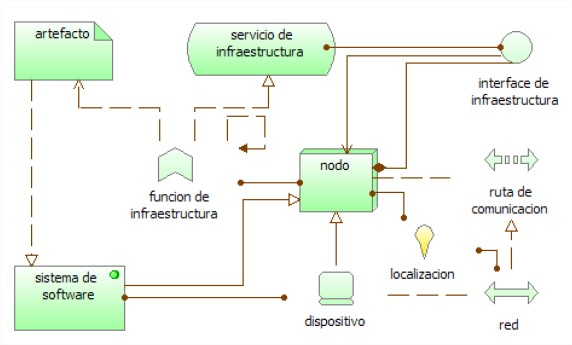
\includegraphics[width=10cm,height=5cm]{arquitectura/tecnologia/imgs/infraestructura-e}
	\caption{Punto de vista de infraestructura}{\scriptsize \textbf{Fuente:} Archimate 2.0 \cite{WEB7}}
\end{figure}

\subsubsection{Caso}

Para el desarrollo de la aplicación se cuenta con un servidor de aplicaciones que permite el despliegue del componente desarrollo, este se encuentra alojado en un hosting que debe ser adquirido por la organización para poder tener acceso público de la aplicación.

%%grafo
\begin{figure}[th!]
	\centering
	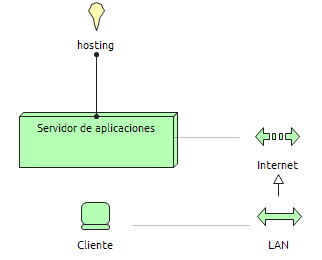
\includegraphics[width=12cm,height=7cm]{arquitectura/tecnologia/imgs/infraestructura}
	\caption{Punto de vista de infraestructura}{\scriptsize \textbf{Fuente:} Imagen propia}
\end{figure}
\newpage

\subsubsection{Punto de Vista de Uso de Infraestructura}

El punto de vista de uso infraestructura permite visualizar las diferentes funciones que se realizan en el entornode la aplicación relacionadas con la infraestructura.

%%grafo

\begin{figure}[th!]
	\centering
	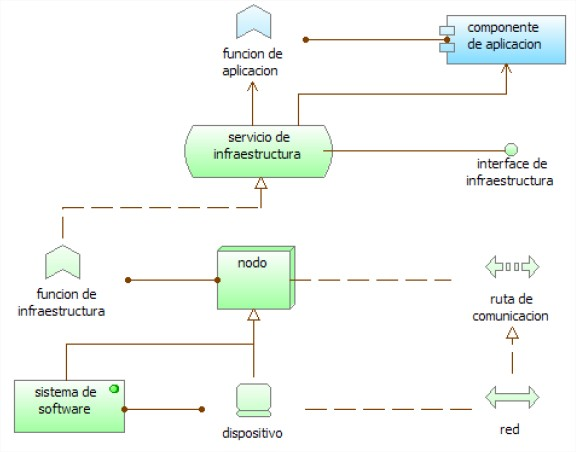
\includegraphics[width=10cm,height=5cm]{arquitectura/tecnologia/imgs/uso-e}
	\caption{Punto de Vista de Uso de Infraestructura}{\scriptsize \textbf{Fuente:} Archimate 2.0 \cite{WEB7}}
\end{figure}

\subsubsection{Caso}

Para el desarrollo de la aplicación se presenta el alojamiento de los componentes y la dependenica que se genera entre ellos.

%%grafo
\begin{figure}[th!]
	\centering
	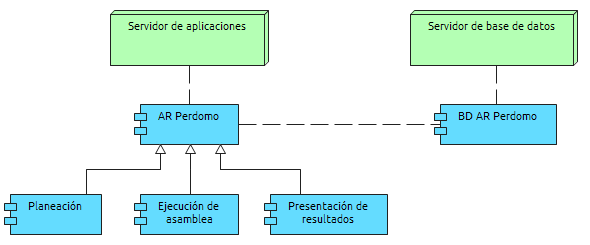
\includegraphics[width=12cm,height=7cm]{arquitectura/tecnologia/imgs/uso}
	\caption{Punto de Vista de Uso de Infraestructura}{\scriptsize \textbf{Fuente:} Imagen propia}
\end{figure}
\newpage

\subsubsection{Punto de Vista de Organización e Implementación}

El punto de vista de Organización e Implementación permite presentar la colaboración entre componentes.

%%grafo

\begin{figure}[th!]
	\centering
	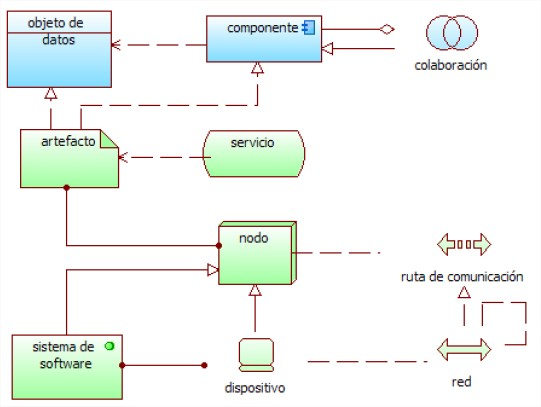
\includegraphics[width=10cm,height=5cm]{arquitectura/tecnologia/imgs/organizacion-e}
	\caption{Punto de Vista de Organización e Implementación}{\scriptsize \textbf{Fuente:} Archimate 2.0 \cite{WEB7}}
\end{figure}

\subsubsection{Caso}

En el diagrama se presenta la colaboración realizada entre componentes para el registro de asambleas, en ello participan el servidor de aplicaciones, el servidor de base de datos y la colaboración entre servicios.

%%grafo
\begin{figure}[th!]
	\centering
	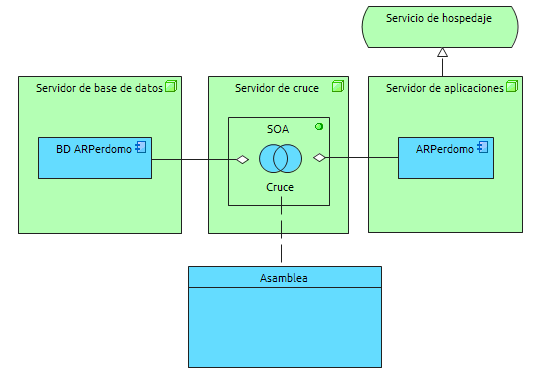
\includegraphics[width=12cm,height=7cm]{arquitectura/tecnologia/imgs/organizacion}
	\caption{Punto de Vista de Organización e Implementación}{\scriptsize \textbf{Fuente:} Imagen propia}
\end{figure}
\newpage